\documentclass{jsarticle}

\usepackage[top=30mm, bottom=36mm, left=28mm, right=28mm]{geometry}
\usepackage[yyyymmdd]{datetime}
\usepackage[dvipdfmx]{graphicx}
\usepackage[subrefformat=parens]{subcaption}
\usepackage{listings}

\makeatletter
\def\maketitle{%
    \null
    \thispagestyle{empty}%
    \vfill
    \begin{center}\leavevmode
        \normalfont
        {\LARGE \@title\par}%
        \vskip 1cm
        {\Large \@author\par}%
        \vskip 1cm
        {\Large \@date\par}%
    \end{center}%
    \vfill
    \null
    \@thanks%\vfil\null
    \cleardoublepage
}
\makeatother

\title{データ解析特論 第10回\\ランキングとその評価}
\author{201720690 小松 弘人}
\date{\today}
\pagestyle{empty}

\begin{document}
\maketitle
\thispagestyle{empty}
\section{課題}

manabaから共著関係ネットワークのデータをダウンロードし、
そのネットワークからその分野における権威を見つける。
このデータには、apscoauthor.csvとcitation\_count.txtの
2ファイルが含まれている。
apscoauthor.csvは、物理学の分野の論文の共著関係ネットワークを
エッジリストで表現したものである。
また、citation\_count.txtは、論文の被引用数であり、
このデータをこの分野における権威度を表す正解データとして用いる。

今回の課題では、共著関係ネットワークにおけるノードの次数および
PageRankによって著者をランキングする。
次に、このランキングを以下の方法を用いて評価を行う。
\begin{enumerate}
    \item
        被引用数に基づくランキングと共著ネットワークに基づく
        ランキングの順位相関係数を求める
    \item
        被引用数上位$1\%$の著者をこの分野の権威であると考え、
        これらの著者を正解データとみなす。
        その場合の、Precision-Recall曲線をplotする
    \item
        被引用数をその著者の適合度とみなし、nDCG@100を計算する
\end{enumerate}

\section{ランキング}
著者のランキングは、各ノードに対して次数中心性 (degree)、
固有ベクトル中心性 (evcent)、PageRank (page.rank) を計算し、
sort関数およびrank関数を用いて行う。

\section{結果}
\subsection{順位相関係数}
順位相関係数には、スピアマンの順位相関係数 (式\ref{eq:s}) と
ケンドールの順位相関係数 (式\ref{eq:k}) が存在する。
\begin{equation}
    \rho = \frac{\sum_i{(x_i-\bar{x})(y_i-\bar{y})}}{\sqrt{\sum_i{(x_i-\bar{x})^2}}\sqrt{\sum_i{(y_i-\bar{y})^2}}}, \\
    \bar{x}=\bar{y}=\frac{1+N}{2}
    \label{eq:s}
\end{equation}
\begin{equation}
    \tau = \frac{2P}{\frac{1}{2}N(N-1)}-1
    \label{eq:k}
\end{equation}
$x_i, y_i$はデータ$i$の順位、$P$は2つのランキングで
順序関係が一致しているデータ組の数、$N$はデータ数を示す。

それぞれのランキングについて順位相関係数を計算した結果を表\ref{tbl:cor}に示す。
\begin{table}[h]
    \centering
    \caption{順位相関係数}
    \label{tbl:cor}
    \begin{tabular}{c|c|c|c} \hline
        順位相関係数 & 次数中心性 & 固有ベクトル中心性 & PageRank \\ \hline \hline
        スピアマンの順位相関係数 & 0.5819306 & 0.2700521 & 0.5887235 \\
        ケンドールの順位相関係数 & 0.4520609 & 0.1905424 & 0.4348009 \\ \hline
    \end{tabular}
\end{table}

\subsection{Precision-Recall曲線}
被引用数 (citation\_count.txt) の上位$1\%$の著者を正解データとみなし、
Precision (式\ref{eq:p})、Recall (式\ref{eq:r}) を計算し、
Precision-Recall曲線を描画した。
\begin{equation}
    P = \frac{|A \cap B|}{|B|}
    \label{eq:p}
\end{equation}
\begin{equation}
    R = \frac{|A \cap B|}{|A|}
    \label{eq:r}
\end{equation}
Precision-Recall曲線を図\ref{img:prcurve}に示す。
\begin{figure}[h]
    \centering
    \begin{tabular}{ccc}
        \begin{subfigure}[h]{.33\linewidth}
            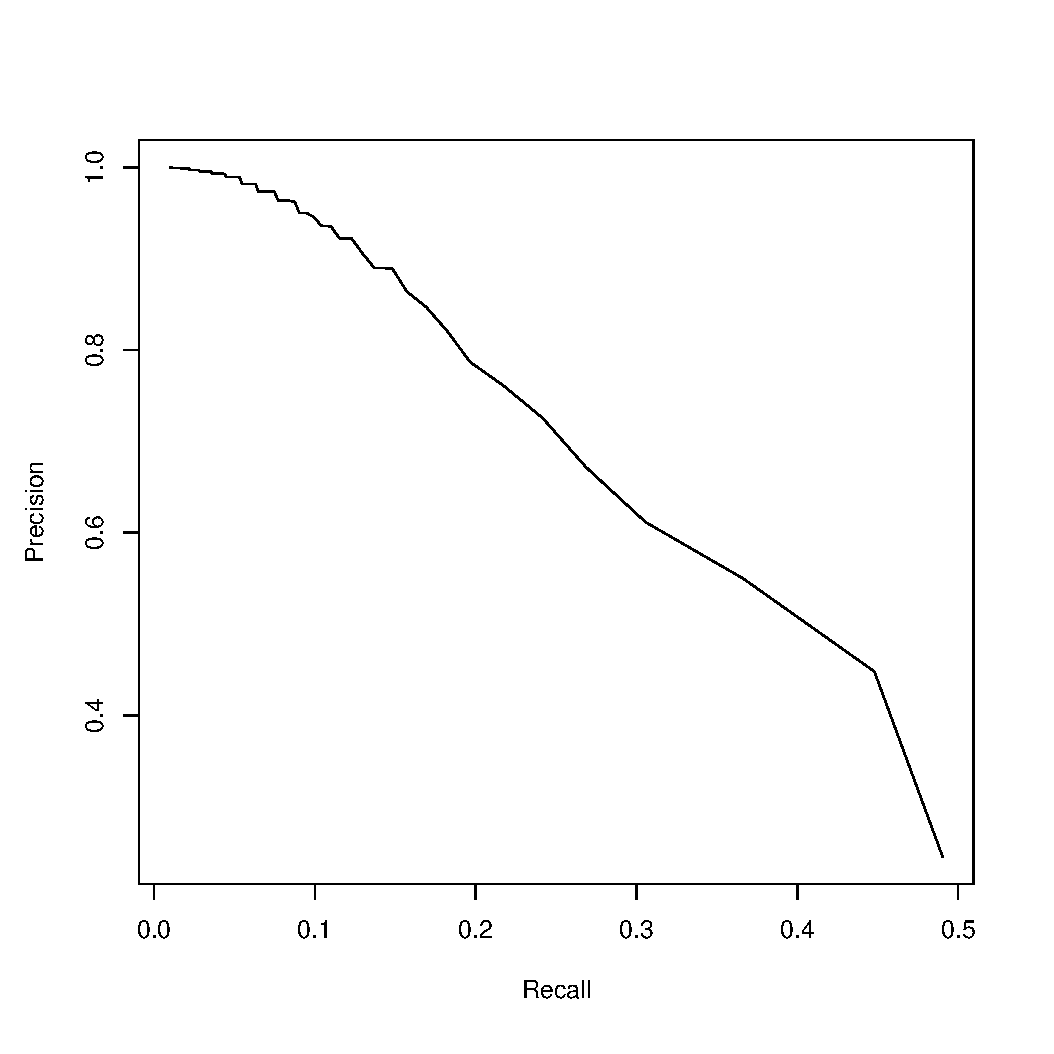
\includegraphics[width=\linewidth]{img/prcurve_d.eps}
            \caption{次数中心性}
        \end{subfigure}
        \begin{subfigure}[h]{.33\linewidth}
            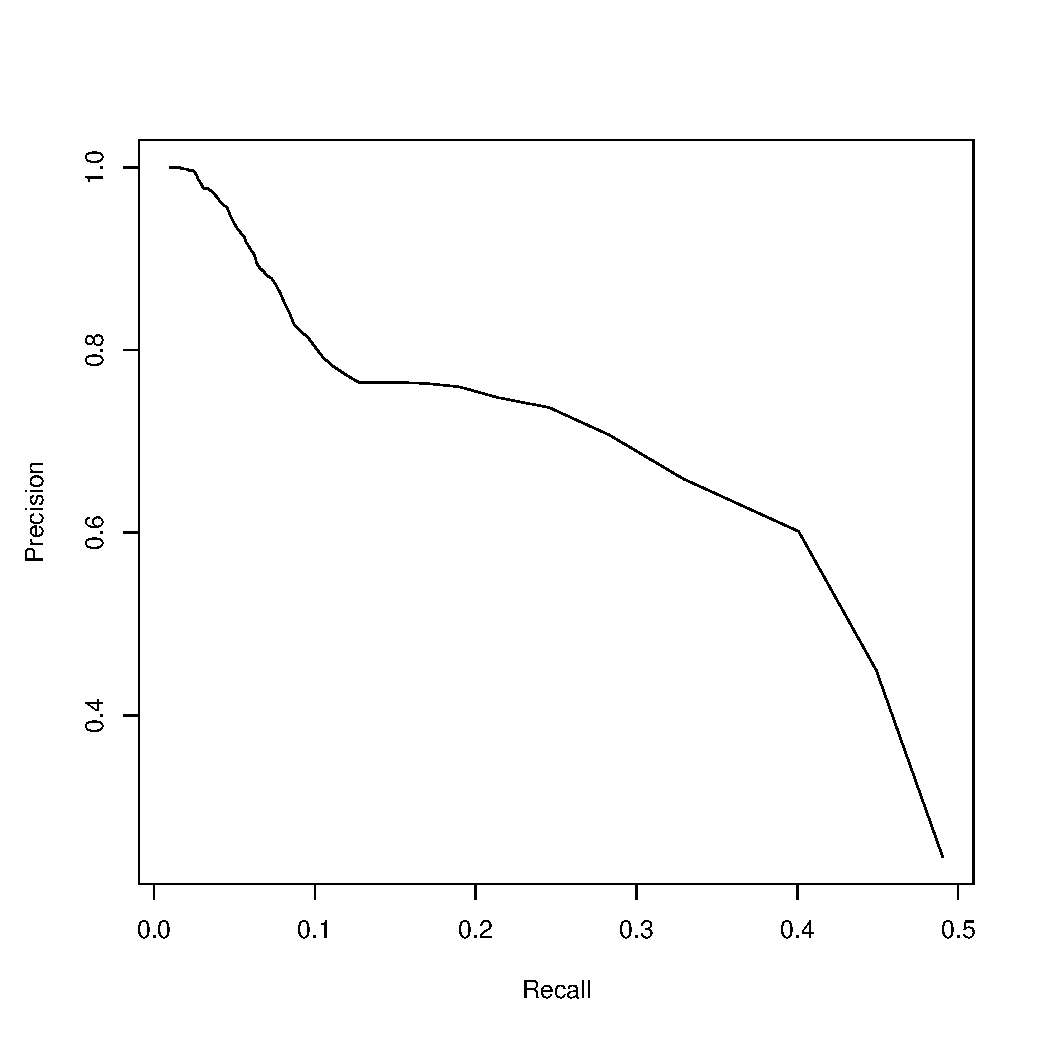
\includegraphics[width=\linewidth]{img/prcurve_e.eps}
            \caption{固有ベクトル中心性}
        \end{subfigure}
        \begin{subfigure}[h]{.33\linewidth}
            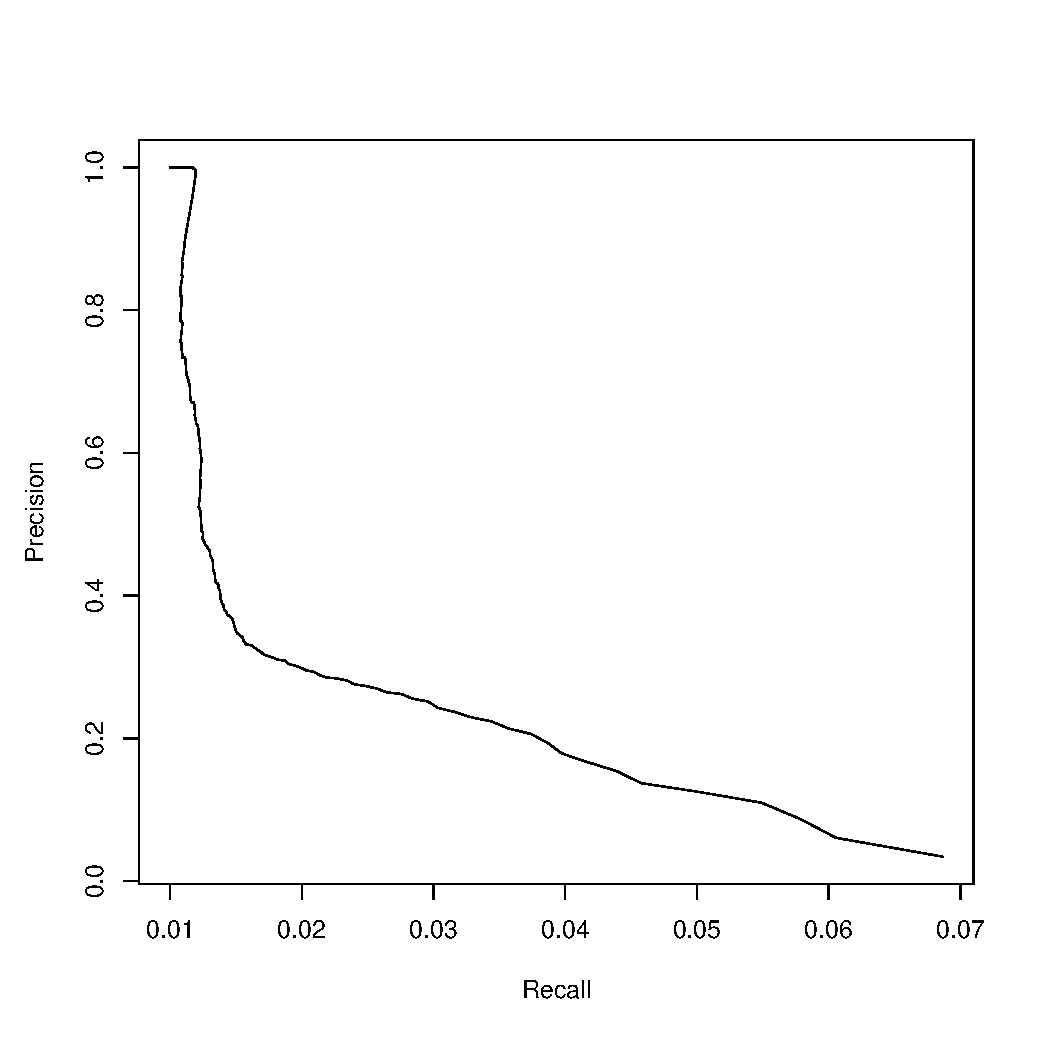
\includegraphics[width=\linewidth]{img/prcurve_p.eps}
            \caption{PageRank}
        \end{subfigure}
    \end{tabular}
    \caption{Precision-Recall曲線}
    \label{img:prcurve}
\end{figure}

\subsection{nDCG@100}
それぞれのランキングについてnDCG (式\ref{eq:nDCG}) を計算した。
適合度はcitation\_count.txtの値を用いる。
結果を表\ref{tbl:nDCG}に示す。
\begin{equation}
    nDCG@k = \frac{\sum_{r=1}^k{\frac{g(r)}{\log{(r+1)}}}}{\sum_{r=1}^k{\frac{g^\star(r)}{\log{r+1}}}}
    \label{eq:nDCG}
\end{equation}
\begin{table}[h]
    \centering
    \caption{nDCG@100}
    \label{tbl:nDCG}
    \begin{tabular}{ccc} \hline
        次数中心性 & 固有ベクトル中心性 & PageRank \\ \hline \hline
        0.2757818 & 0.2574463 & 0.2529339 \\ \hline
    \end{tabular}
\end{table}

\section{考察}
それぞれの評価指標における各ランキングの評価をまとめると、
スピアマンの順位相関係数ではPageRank、次数中心性、固有ベクトル中心性、
ケンドールの順位相関係数では次数中心性、PageRank、固有ベクトル中心性の順に
評価が高かった。
また、Precision-Recall曲線を見ると、原点周りの面積が大きいのは
次数中心性、固有ベクトル中心性、PageRankの順だった。
nDCG@100では、次数中心性、固有ベクトル中心性、PageRankの順であった。
これらの評価指標を統合して考えると、次数中心性を基にランキングした結果が
今回の問題においては最も正解に近いランキングを行えていたことが分かった。

PageRankと固有ベクトル中心性については、順位相関係数においてはPageRankの方が大きく、
Precision-Recall曲線およびnDCG@100は固有ベクトル中心性の方が良いことから、
ランキング全体の一致度はPageRankでランキングを行った場合の方が高いが、
ランキング上位のデータの適合度については固有ベクトル中心性の方が良いという結果になった。

\section{スクリプト}
\begin{lstlisting}[basicstyle=\ttfamily\footnotesize, frame=single]
library(igraph)

# データの読み込み
g = read.graph('data/apscoauthor.csv')
answer = read.table('data/citation_count.txt')

# ランキング
## 次数中心性の計算
d = degree(g)
## 固有ベクトル中心性の計算
e = evcent(g)$vector
## PageRankの計算
p = page.rank(g)$vector

## ランキングの作成
ans = sort(answer$V2, decreasing = TRUE, method = "s", index.return = TRUE)
ans_rnk = rank(-answer$V2)
res_d = sort(d, decreasing = TRUE, method = "s", index.return = TRUE)
res_d_rnk = rank(-d)
res_e = sort(e, decreasing = TRUE, method = "s", index.return = TRUE)
res_e_rnk = rank(-e)
res_p = sort(p, decreasing = TRUE, method = "s", index.return = TRUE)
res_p_rnk = rank(-p)

## 順位相関係数
### スピアマン
rho_d = (cor.test(ans_rnk, res_d_rnk, method="s"))$estimate; rho_d
rho_e = (cor.test(ans_rnk, res_e_rnk, method="s"))$estimate; rho_e
rho_p = (cor.test(ans_rnk, res_p_rnk, method="s"))$estimate; rho_p

### ケンドール
tau_d = (cor.test(ans_rnk, res_d_rnk, method="k"))$estimate; tau_d
tau_e = (cor.test(ans_rnk, res_e_rnk, method="k"))$estimate; tau_e
tau_p = (cor.test(ans_rnk, res_p_rnk, method="k"))$estimate; tau_p

## precision--recall curve
A = ans$ix[1:(length(ans$ix)*0.01)]
seg = 200

P_d = c(); R_d = c()
for (i in 0:seg) {
    q = 100*i/seg
    B = res_d$ix[1:(length(ans$ix)*q/100)]
    AandB = intersect(A, B)
    P_d[i] = length(AandB) / length(B)
    R_d[i] = length(AandB) / length(A)
}
plot(P_d, R_d, type="l", xlab="Recall", ylab="Precision")

P_e = c(); R_e = c()
for (i in 0:seg) {
    q = 100*i/seg
    B = res_e$ix[1:(length(ans$ix)*q/100)]
    AandB = intersect(A, B)
    P_e[i] = length(AandB) / length(B)
    R_e[i] = length(AandB) / length(A)
}
plot(P_e, R_e, type="l", xlab="Recall", ylab="Precision")

P_p = c(); R_p = c()
for (i in 0:seg) {
    q = 100*i/seg
    B = res_p$ix[1:(length(ans$ix)*q/100)]
    AandB = intersect(A, B)
    P_p[i] = length(AandB) / length(B)
    R_p[i] = length(AandB) / length(A)
}
plot(P_p, R_p, type="l", xlab="Recall", ylab="Precision")

## nDCG@100
k = 100

### 理想的なランキングにおける値
isum = 0
for(r in 1:k) {
    isum = isum + ans$x[r] / log(r+1)
}

dsum = 0
for(r in 1:k) {
    dsum = dsum + answer$V2[res_d$ix[r]] / log(r+1)
}

esum = 0
for(r in 1:k) {
    esum = esum + answer$V2[res_e$ix[r]] / log(r+1)
}

psum = 0
for(r in 1:k) {
    psum = psum + answer$V2[res_p$ix[r]] / log(r+1)
}

(dsum/isum)
(esum/isum)
(psum/isum)
\end{lstlisting}

\end{document}
